\documentclass[11pt,reqno]{amsart}
\usepackage[top=1in, left=1in, right=1in, bottom=1in]{geometry}                % See geometry.pdf to learn the layout options. There are lots.
\geometry{letterpaper}                   % ... or a4paper or a5paper or ...
\usepackage[parfill]{parskip}    % Activate to begin paragraphs with an empty line rather than an indent
%\usepackage{algorithm, algorithmic}

\usepackage{algorithm}
\usepackage{algpseudocode}

\usepackage{graphicx}

\usepackage{verbatim}
\usepackage{amssymb}
\usepackage{amsmath}

\usepackage{enumitem}

\usepackage{setspace}
\doublespacing

\usepackage{natbib}

%\usepackage{epstopdf}
%\DeclareGraphicsRule{.tif}{png}{.png}{`convert #1 `dirname #1`/`basename #1 .tif`.png}

\newcommand{\RR}{I\!\!R} %real numbers
\DeclareMathOperator{\diag}{diag}

\algnewcommand{\Inputs}[1]{%
  \State \textbf{Inputs:}
  \Statex \hspace*{\algorithmicindent}\parbox[t]{.8\linewidth}{\raggedright #1}
}
\algnewcommand{\Initialize}[1]{%
  \State \textbf{Initialize:}
  \Statex \hspace*{\algorithmicindent}\parbox[t]{.8\linewidth}{\raggedright #1}
}

\title[RVD3]{RVD3: Variant detection model with improved robustness and accuracy for low-depth targeted next-generation sequencing data}
\author{}
%\date{}                                           % Activate to display a given date or no date

\begin{document}

\begin{abstract}
Sensitivity analysis Bayesian model
Jeffreys prior improves robustness and accuracy of Single Nucleotide Variant detection algorithm.

\end{abstract}

\maketitle

%%%%%%%%%%%%%%%%%%
% Introduction
%%%%%%%%%%%%%%%%%%
\section{Introduction}





%%%%%%%%%%%%%%%%%%
% Data Sets
%%%%%%%%%%%%%%%%%%
\section{Data Sets}

\subsection{Synthetic DNA Sequence Data}

Two 400bp DNA sequences that are identical except at 14 loci with variant bases were synthesized and clonally isolated and labeled case and control. Sample of the case and control DNA were mixed at defined fractions to yield defined minor allele frequencies (MAFs) of 0.1\%, 0.3\%, 1\%, 10\%, and 100\%. More details of the experimental protocol are available from the original publication~\citep{Flaherty:2011ja}. We aligned the reads to the reference sequence using BWA v0.7.4 with the -C50 option to filter for high mapping quality reads.

To simulate lower coverage data while retaining the error structure of real NGS data, BAM files for the synthetic DNA data were downsampled $10\times$, $100\times$, $1,000\times$, and $10,000\times$ using Picard v1.96. The final data set contains read pairs for three replicates of each case and pairs of reads three replicates for the control sample giving $N=6$ replicates for the control and each MAF level.

\subsection{Yeast Data}


%%%%%%%%%%%%%%%%%%
% RVD3 Model
%%%%%%%%%%%%%%%%%%
\section{RVD3 Model}

\subsection{Model Structure}\label{sec:model_structure}
RVD3 is based on a hierarchical Bayesian model. Through hypothesis test on case and control samples by RVD3, we can call the variants sucsessfully. Now the definitions for sample data are given: $r_{ji}$ is the number of reads with a non-reference base at position $j$ in replicate $i$, and $n_{ji}$ is the total number of reads at position $j$ in replicate $i$. Three hyperparameters are:  $\mu_0$, a global error rate; $M_0$, a global precision; $M_j$, a local precision; $\mu_0$, the global error rate expected across all positions; $M_0$, the global position which estimates the variation in the error rate across the positioins. $M_j$, the local precision measures the alteration in the error rate across replicates at position $j$.
RVD3 hierarchically includes four levels of samplings:  $r_{ji} | n_{ji} \thicksim \text{Binomial}(\theta_{ji}, n_{ji})$ models the variation due to sampling the pool of DNA molecules on the sequencer. $\theta_{ji} \thicksim \text{Beta}(\mu_j, M_j)$ models the variation caused by experimental repeatability. The variation in error rate due to sequence context is modeled by $\mu_j \thicksim \text{Beta}(\mu_0, M_0)$. Two kinds of priors for $M_{j}$ are Log-normal prior and Jeffreys prior, which enhanced the former RVD model [XX]. $ M_{j} \thicksim \text{log-normal}(\mu, \sigma)$ is the model for Log-normal prior, and $pi\left({M}_{j}\right)$ for Jeffreys prior is based on Fisher information. The graphical chart for RVD3 with different priors are shown in Figure~\ref{fig:graphical_model}.

\begin{figure}[h]
\begin{center}
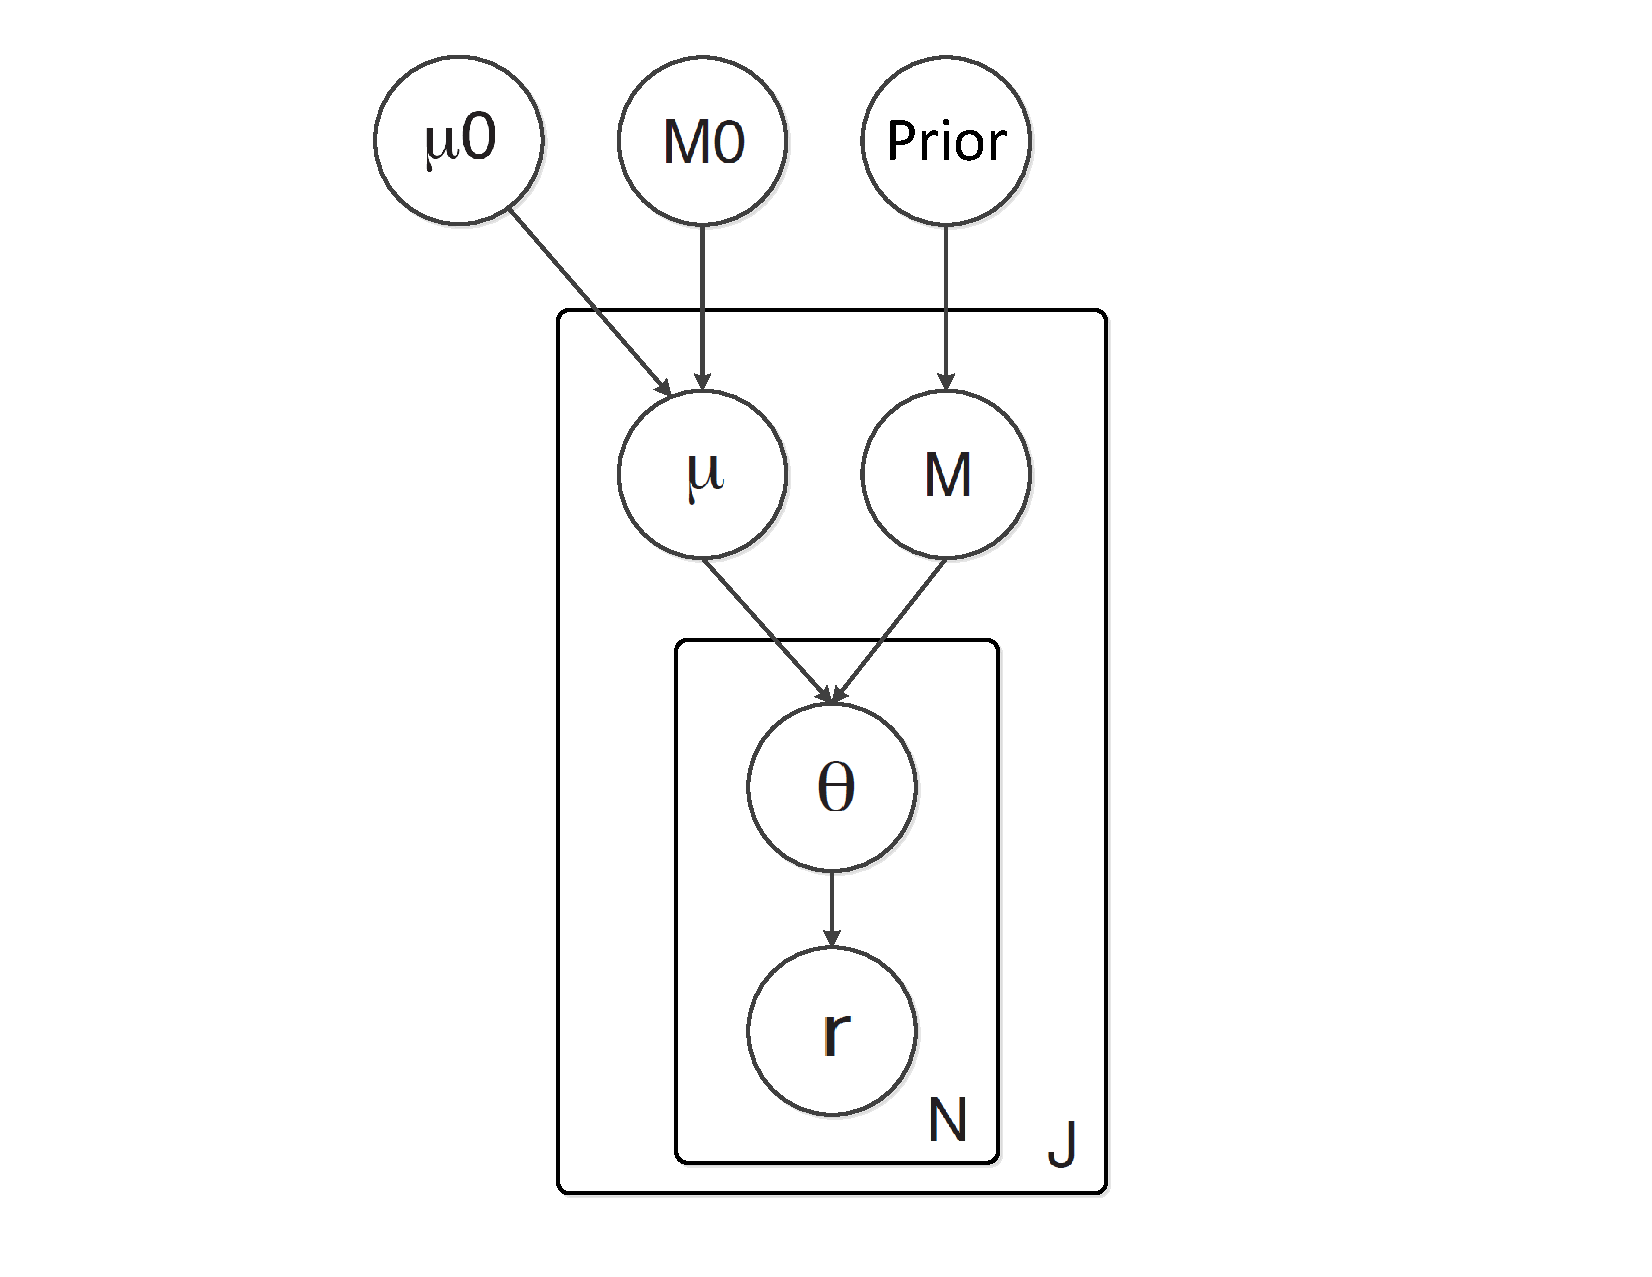
\includegraphics[width=40mm]{figs/RVD3_model.pdf}
\caption{RVD3 Graphical Model}
\label{fig:graphical_model}
\end{center}
\end{figure}


%%%%%%%%%%%%%%%%%%
% Inference & Hypothesis Testing
%%%%%%%%%%%%%%%%%%
\subsection{Inference and Hypothesis Testing}

The primary object of inference in this model is the joint posterior distribution function over the latent variables,
\begin{equation}
	p(\mu, \theta | r, n; \phi)  = \frac{ p(\mu, \theta, r | n; \phi) } {p ( r | n; \phi)},
\end{equation}
where the parameters are $\phi \triangleq \{\mu_0, M_0, M\}$.

The Beta distribution over $\mu_j$ is conjugate to the Binomial distribution over $\theta_{ji}$, so we can write the posterior distribution as a Beta distribution. However, there is not a closed form for the product of a Beta distribution with another Beta distribution, so exact inference is intractable.

Instead, we have developed a Metropolis-within-Gibbs  approximate inference algorithm shown in Algorithm~\ref{alg:metro_gibbs}. First, the hyperparameters are initialized using method-of-moments (MoM). Given those hyperparameter estimates, we sample from the marginal posterior distribution for $\mu_j$ given its Markov blanket using a Metropolis-Hasting rejection sampling rule. Finally, we sample from the marginal posterior distribution for $\theta_{ji}$ given its Markov blanket. Samples from $\theta_{ji}$ can be drawn from the posterior distribution directly  because the prior and likelihood form a conjugate pair. This sampling procedure is repeated until the chain converges to a stationary distribution then we draw samples from the posterior distribution over latent variables.

\begin{algorithm}[ht]
\caption{Metropolis-within-Gibbs Algorithm}
\label{alg:metro_gibbs}
\begin{algorithmic}[1]

\State Initialize $\theta$, $\mu$, $M$, $\mu_0$, $M_0$
\Repeat
\For {each location j} \Comment{Sample $\mu_j$}
  \State Draw T samples from $p \left( \mu_j |\theta_{ij},\mu_0,M_0\right)$ using M--H
  \State Set $\mu_j$ to the sample median for the T samples


  \For {each replicate i} \Comment{Sample $\theta_{ji}$}
	\State Sample from $p \left( \theta_{ij} |r_{ij},n_{ij},\mu_j,M \right)$
  \EndFor

\EndFor
\Until {sample size sufficient}
\end{algorithmic}
\end{algorithm}

%%%%%%%%%%%%%
% Initialization
%%%%%%%%%%%%%
\subsubsection{Initialization}
The initial values for the model parameters and latent variables is obtained by a method-of-moments (MoM) procedure. MoM works by setting the population moment equal to the sample moment. A system of equations is formed such that the number of moment equations is equal to the number of unknown parameters and the equations are solved simultaneously to give the parameter estimates. We simply start with the data matrices $r$ and $n$ and work up the hierarchy of the graphical model solving for the parameters of each conditional distribution in turn.

We present the initial parameter estimates here and provide the derivations in Appendix~\ref{sec:appendix_mom}. The MoM estimate for replicate-level parameters are
$\tilde{\theta}_{ji} = \frac{r_{ji}} {n_{ji}}$.
The estimates for the position-level parameters are
$\tilde{\mu}_j = \frac{1}{N} \sum_{i=1}^N \theta_{ji}$
and
$\tilde{M_j} = \frac{ \tilde{\mu}_j (1 - \tilde{\mu}_j ) } { \frac{1}{N} \sum_{i=1}^N \theta_{ji}^2 } -1$.
The estimates for the genome-level parameters are
$\tilde{\mu}_0 = \frac{1}{J} \sum_{j=1}^J \mu_j$
and
$\tilde{M}_0 = \frac{ \tilde{\mu}_0 (1 - \tilde{\mu}_0 ) } {\frac{1}{J} \sum_{j=1}^J \mu_j^2 } -1$.
While MoM is known to have the potential to return estimates outside the true parameter bounds, we have not encountered such behavior in this application.

%%%%%%%%%%%%%%%%%%
% Sampling theta
%%%%%%%%%%%%%%%%%%
\subsubsection{Sampling from $p \left( \theta_{ij} |r_{ij},n_{ij},\mu_j,M \right)$}

Samples from the posterior distribution
$p(\theta_{ji} | r_{ji}, n_{ji}, \mu_j, M_j)$
are drawn analytically because of the Bayesian conjugacy between the prior
$p(\theta_{ji} | \mu_j, M_j) \thicksim \text{Beta}(\mu_j, M_j)$
and the likelihood
$p(r_{ji} | n_{ji}, \theta_{ji}) \thicksim \text{Binomial}(\theta_{ji}, n_{ji})$.
The posterior distribution is
\begin{equation}
	p(\theta_{ji} | r_{ji}, n_{ji}, \mu_j, M_j) \thicksim \text{Beta}\left( \frac{r_{ji} + M_j \mu_j}{n_{ji} + M_j} , n_{ji} + M_j\right).
\end{equation}

%%%%%%%%%%%%%%%%%%
% Sampling mu
%%%%%%%%%%%%%%%%%%
\subsubsection{Sampling from $p \left( \mu_j |\theta_{ji},M_j,\mu_0,M_0\right)$}
The posterior distribution over $\mu_j$ given its Markov blanket is
\begin{equation}
	p( \mu_j | \theta_{ji}, M_j, \mu_0, M_0 ) \propto p(\mu_j | \mu_0, M_0) p(\theta_{ji} | \mu_j, M_j).
\end{equation}

Since the prior, $p(\mu_j | \mu_0, M_0)$, is not conjugate to the likelihood, $p(\theta_{ji} | \mu_j, M_j)$, we cannot write an analytical form for the posterior distribution. Instead, we sample from the posterior distribution using the Metropolis-Hastings algorithm.

A candidate sample is generated from the symmetric proposal distribution $Q(\mu_j^* | \mu_j^{(p)}) \thicksim \mathcal{N}(\mu_j^{(p)}, \sigma_j^2)$, where $\mu_j^{(p)}$ is the $p$th from the posterior distribution. The acceptance probability is then
\begin{equation}
	a = \frac{ p(\mu_j^* | \mu_0, M_0) p(\theta^{(p+1)}_{ji} | \mu_j^*, M_j) } {p(\mu_j^{(p)} | \mu_0, M_0) p(\theta^{(p+1)}_{ji} | \mu_j^{(p)}, M_j)}
\end{equation}

We fixed the proposal distribution variance for all the Metropolis-Hastings steps within a Gibbs iteration to $\sigma_j = 0.1 \cdot \mu_j^{(p)}$ if $\mu_j^{(p)} \in (10^{-3},1-10^{-3})$; otherwise, we set $\sigma_j = 10^{-4}$ if $\mu_j^{(p)}< 10^{-3}$ and $\sigma_j = 10^{-1}-10^{-4}$ if $\mu_j^{(p)}>1-10^{-3}$. Though it is not theoretically necessary, we have found that the algorithm performance improves when we take the median of five or more M-H samples as a single Gibbs step for each position.


We resample from the proposal if the sample is outside of the support of the posterior distribution. We typically discard 20\% of the sample for burn-in and thin the chain by a factor of 2 to reduce autocorrelation among samples. Since, each position $j$ is exchangeable given the global hyperparameters $\mu_0$ and $M_0$ this sampling step can be distributed across up to $J$ processors.

%%%%%%%%%%%%%%%%%%
% Sampling Mj
%%%%%%%%%%%%%%%%%%
\subsubsection{Sampling from $p \left( M_{j} |\mu,\sigma, \theta_{ji},\mu_j\right)$}
For Jeffreys prior,since ${\theta }_{ji}\sim Beta\left( {\mu }_{j},{M}_{j}\right)$, the Fisher information is given by

\begin{equation}\label{equ:JefferyInference}
I\left({M}_{j}\right)={E}_{{M}_{j}}\left[ -\frac{\delta ^{2}\log p\left(\theta _{j}|\mu_{j},M_{j}\right)}{\delta M^{2}_{j}}\right]
\end{equation}

Now to calculate the equations to acquire the Fisher information, we assume there is only one replicate,

\begin{equation}\label{eqn:Betapdf}
p\left({\theta }_{j} \right)= \frac{\Gamma \left({M}_{j} \right)}{\Gamma \left({\mu }_{j} {M}_{j}\right)\Gamma \left(( 1-{\mu }_{j}){M}_{j}\right)} {{\theta}_{j}}^{{\mu}_{j}{M}_{j}-1}{\left(1-\theta\right)_{j}}^{\left(1-{\mu}_{j}\right){M}_{j}-1}
\end{equation}

\begin{equation}\label{equ:JefferyInference1}
\begin{split}
\log p\left(\theta_{j}|\mu_{j},M_{j}\right)& =\log \Gamma \left(M_{j}\right)-\log \Gamma\left(\mu_{j},M_{j}\right)- \log \Gamma\left(1-\mu_{j},M_{j}\right)\\
& + (\mu_{j}M_{j}-1)\log\theta_{j} + ((1-\,u_{j})M_{j}-1)\log(1-\theta_{j})\
\end{split}
\end{equation}

\begin{equation}
\frac{\delta\log p(\theta_{j})}{\delta M_{j}} = \Psi(M_{j}) - \Psi(\mu_{j} M_{j})\mu_{j} - \Psi((1-\mu_{j})M_{j})(1-\mu_{j}) +\mu_{j}\log\theta_{j} + (1-\mu_{j})\log(1-\theta_{j})
\end{equation}

\begin{equation}
\frac{\delta^{2}\log p(\theta_{j})}{\delta M_{j}^{2}}  = \Psi_{1}(M_{j}) - \Psi_{1}(\mu_{j} M_{j})\mu_{j}^{2} - \Psi_{1}((1-\mu_{j})M_{j})(1-\mu_{j})^{2}
\end{equation}

Now we have the Jeffreys' prior for $M_{j}$:

\begin{equation}
\pi\left({M}_{j}\right) = [-\left(\Psi_{1}(M_{j}) - \Psi_{1}(\mu_{j} M_{j})\mu_{j}^{2} - \Psi_{1}((1-\mu_{j})M_{j}){(1-\mu_{j})^{2}}\right)]^{\frac{1}{2}}
\end{equation}

For log-normal prior, the posterior distribution over $M_{j}$ given its Markov blanket is

\begin{equation}
	p( M_{j} |\mu, \sigma, \theta_{ji},\mu_j) \propto p(\theta_{ji} | \mu_j, M_j) p(M_{j} | \mu, \sigma)
\end{equation}

We have $ \theta_{ji}\thicksim\text{Beta}(\mu_{j},M_{j})$, and $ M_{j} \thicksim \text{log-normal}(\mu, \sigma)$. Since we cannot give an analytical form for this, so we sample from the posterior distribution using the Metropolis-Hastings algorithm.


%%%%%%%%%%%%%%%%%%
% Posterior Density Test
%%%%%%%%%%%%%%%%%%
\subsubsection{Posterior Density Test}\label{sec:hypothesis_test}
Metropolis-within-Gibbs provides samples from the posterior distribution of $\mu_j$ given the case or control data. For notational simplicity, we define the random variables associated with these two distributions $\tilde{\mu}_j^{\text{case}}$ and $\tilde{\mu}_j^{\text{control}}$.

A variant is called if $\tilde{\mu}_j^{\text{case}} > \tilde{\mu}_j^{\text{control}}$ with high confidence,
\begin{equation}\label{eqn:bayes_test}
	\Pr( \tilde{\mu}_j^{\text{case}} - \tilde{\mu}_j^{\text{control}} \geq \tau ) > 1-\alpha,
\end{equation}
where $\tau$ is a detection threshold and $1-\alpha$ is a confidence level. We draw a sample from the posterior distribution $\tilde{\mu}_j^{\Delta} \triangleq \tilde{\mu}_j^{\text{case}} - \tilde{\mu}_j^{\text{control}}$ by simple random sampling with replacement from $\tilde{\mu}_j^{\text{case}}$ and $\tilde{\mu}_j^{\text{control}}$.

The threshold, $\tau$, may be set to zero or optimized for a given median depth and desired MAF detection limit. The optimal $\tau$ minimizes the sum of the false negative rate and false positive rate or, equivalently,  the $L_1$ distance to perfect classification in the ROC curve plot,
\begin{equation}
	\tau^* = \arg\min_\tau \left\{ (1-\text{TPR}(\tau)) + \text{FPR}(\tau) \right\}.
\end{equation}

While we are able to compute the optimal $\tau$ threshold for a test data set, in general we would not have access to $\tau^*$. With sufficient training data, one would be able to develop a lookup table or calibration curve to set $\tau$ based on read depth and MAF level of interest. Absent this information we set $\tau = 0$.


%%%%%%%%%%%%%%%%%%
% Chi^2 Test
%%%%%%%%%%%%%%%%%%
\subsubsection{$\chi^2$ test for non-uniform base distribution}

An abundance of non-reference bases at a position called by the posterior density test may be due to a true mutation or due to a random sequencing error; we would like to differentiate these two scenarios. We assume non-reference read counts caused by a non-biological mechanism results in a uniform distribution over three non-reference bases. In contrast, the distribution of counts among three non-reference bases caused by biological mutation would not be uniform.

We use a $\chi^2$ goodness-of-fit test on a multinomial distribution over the non-reference bases to distinguish these two possible scenarios. The null hypothesis is $H_0: p = (p_1, p_2, p_3)$ where $p_1=p_2=p_3=1/3$. Cressie and Read (1984) identified a power-divergence family of statistics, indexed by $\lambda$, that includes as special cases Pearson's $\chi^2 (\lambda = 1)$ statistic, the log likelihood ratio statistic $(\lambda = 0)$, the Freeman-Tukey statistic $(\lambda = -1/2)$, and the Neyman modified statistic $X^2 (\lambda = -2)$. The test statistic is

\begin{equation}
 2nI^\lambda = \frac{2}{\lambda(\lambda+1)}\sum_{k=1}^3 r_{ji}^{(k)} \left[\left(\frac{r_{ji}^{(k)}}{E_{ji}^{(k)}}\right)^\lambda-1\right];\lambda \in R,
\end{equation}

where $r_{ji}^{(k)}$ is the observed frequency for non-reference base $k$ at position $j$ in replicate $i$ and $E_{ji}^{(k)}$ is the corresponding expected frequency under the null hypothesis. \citet{Cressie1984} recommended $\lambda = 2/3$ when no knowledge of the alternative distribution is available and we choose that value.

We control for multiple hypothesis testing in two ways. We use Fisher's combined probability test \citep{} to combine the p-values for $N$ replicates into a single p-value at position $j$,

\begin{equation}\label{eqn:fisher_combined}
	X_j^2 = -2 \sum_{i=1}^N \ln(p_{ji}).
\end{equation}

Equation~\eqref{eqn:fisher_combined} gives a test statistic that follows a $\chi^2$ distribution with $2N$ degrees of freedom when the null hypothesis is true. Finally, we use the Bejamini-Hochberg method to control the family-wise error rate (FWER) over positions that have been called by the Bayesian hypothesis test~\eqref{eqn:bayes_test} \citep{benjamini1995controlling, efron2010large}.

%%%%%%%%%%%%%%%%%%%%%%%%
% Priors for precision parameter
%%%%%%%%%%%%%%%%%%%%%%%%
\subsection{Priors for precision parameter}
\subsubsection{Improper Prior}
Playing no prior on M is an implicit improper prior. So we coniderated about two typical priors: noninformation prior - Jeffreys prior, and information prior - log-normal prior.

\subsubsection{Jeffreys Prior}
Jeffreys prior is proposed for invariance by Harold Jeffreys (1946), and defined in terms of the Fisher information. For our ploblem,
\begin{equation}\label{eqn:JefferyPrior}
\pi\left({M}_{j}\right)= I\left({M}_{j}\right)^{\frac{1}{2}}
\end{equation}

\subsubsection{Log-normal Prior}
In log-normal distribution, the parameters denoted $\mu$ and $\sigma$, the mean and standard deviation respectively. Log-normal prior was used on $ M_{j}$.
Incorporate lognormal prior on $M_{j}$.


%%%%%%%%%%%%%%%%%%
% Results
%%%%%%%%%%%%%%%%%%
\section{Results}

%%%%%%%%%%%%%%%%%%
% Sensitivity analysis of priors
%%%%%%%%%%%%%%%%%%
\subsection{Sensitivity analysis of priors}
In order to examine the robustness of RVD3 to changes of different priors, we performed information prior (Log-normal) and noninformation prior (Jeffreys).

We found that RVD3 is robust to changing the priors.
The RVD3 algorithm provides estimates of model parameters and latent variables given the data. We show several of these parameters in Figure~\ref{fig:M_jeffrey} and Figure ~\ref{fig:M_lognormal}.

The left column of Figure~\ref{fig:M_jeffrey} and Figure~\ref{fig:M_lognormal} show the read depth for each of the six bam files (three replicates each with two read pairs) for each data set. Because the DNA was not sheared and ligated prior to sequencing, the read depth drops to zero at the boundaries. For the 100\% mutant data set, the read depth drops at the mutant locations. This is due to the parameters imposed at the alignment stage.

\begin{figure}[htbp]
\begin{center}
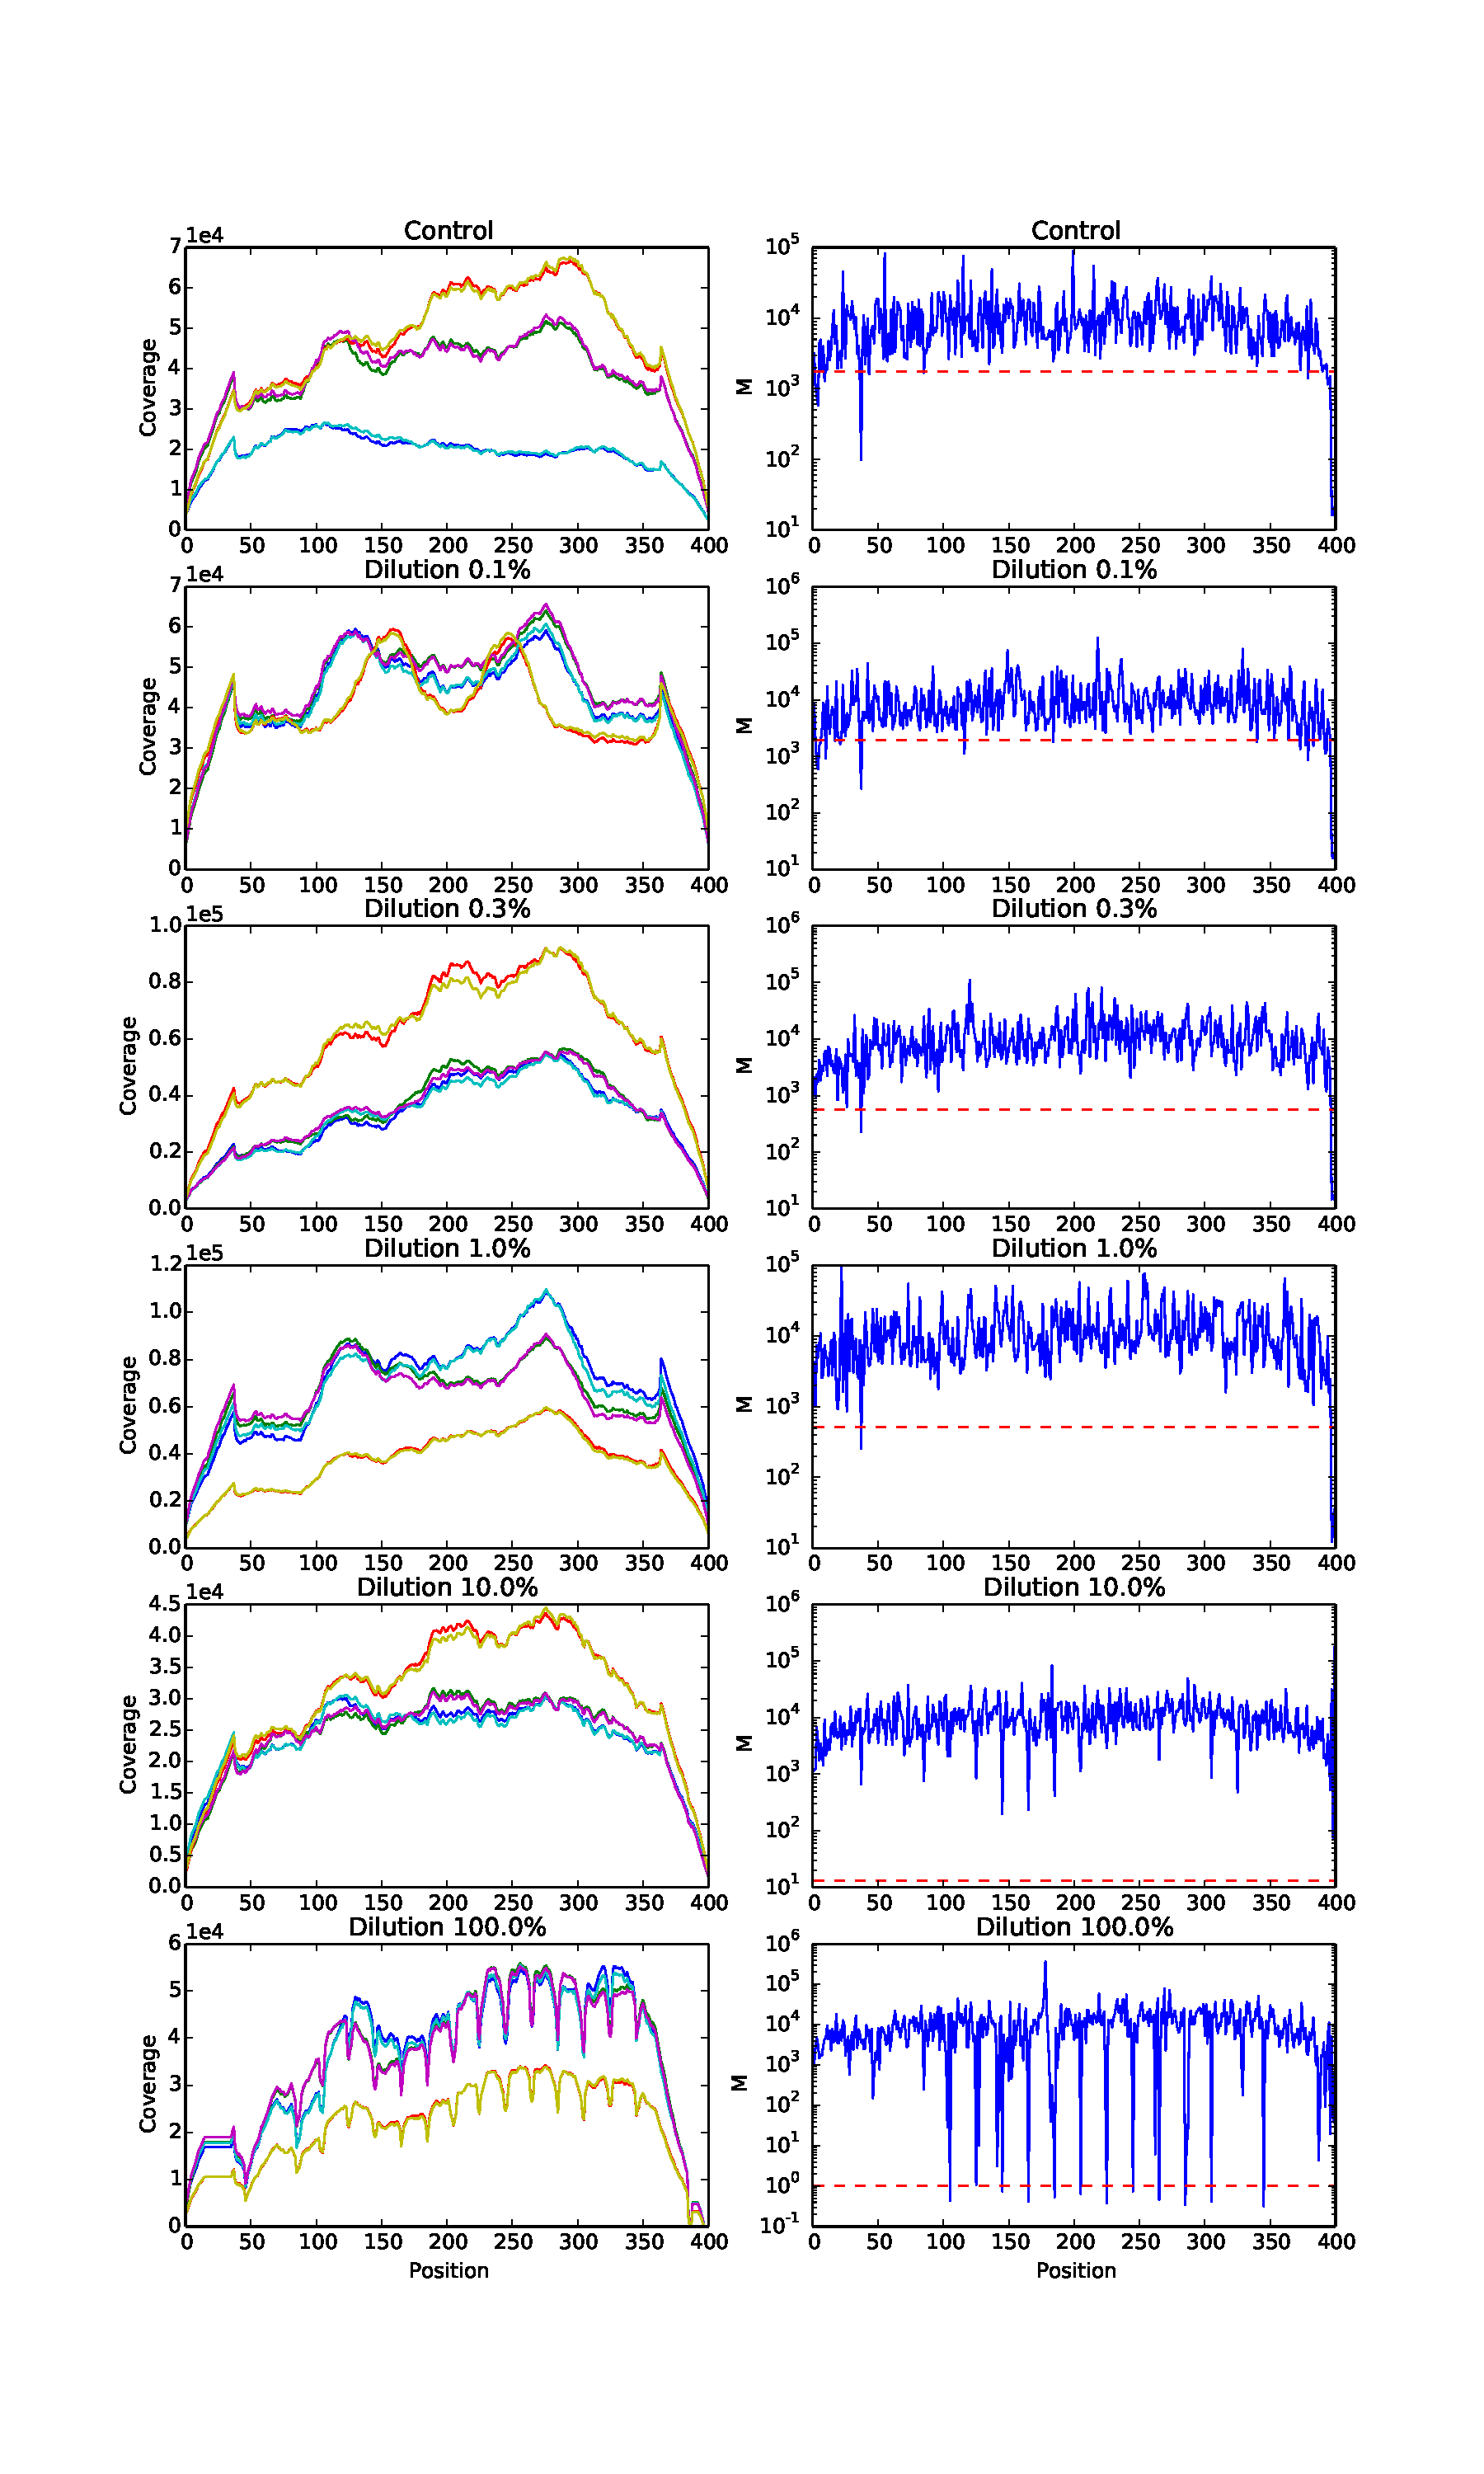
\includegraphics[width=120mm]{figs/M_jeffrey.pdf}
\caption{Key parameters for RVD3 model with Jeffreys prior for synthetic DNA data sets.}
\label{fig:M_jeffrey}
\end{center}
\end{figure}

\begin{figure}[htbp]
\begin{center}
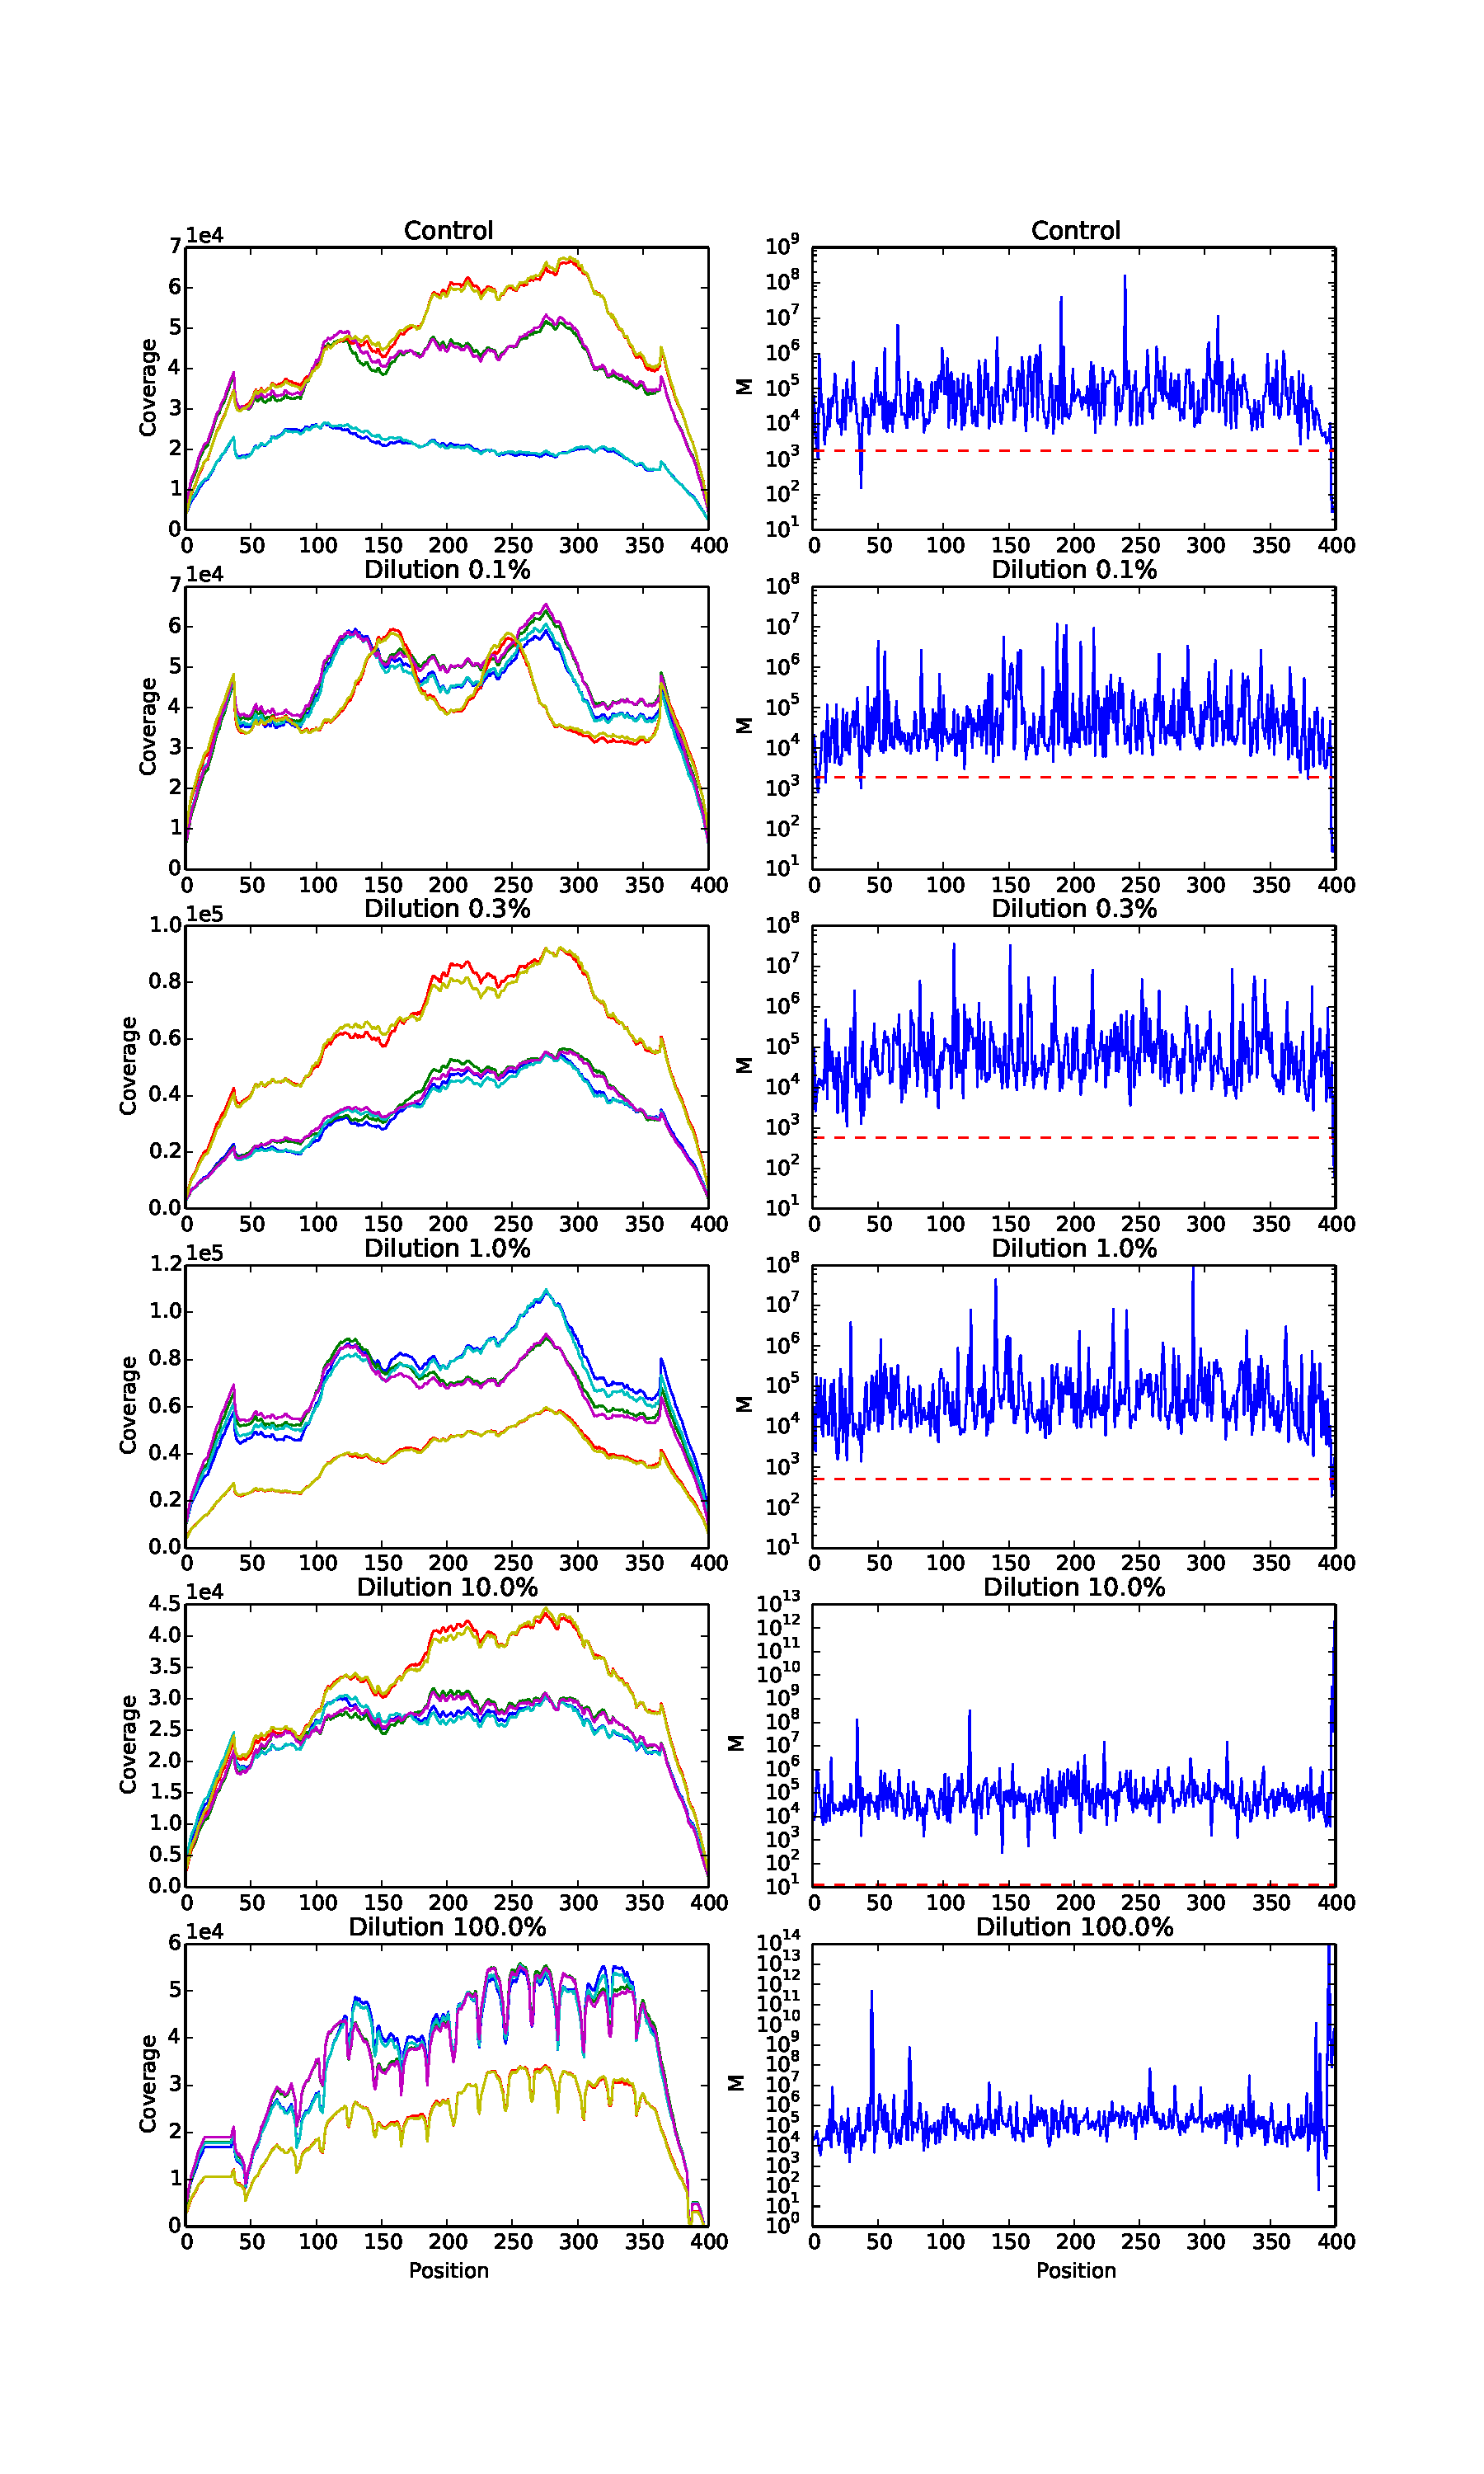
\includegraphics[width=120mm]{figs/M_lognormal.pdf}
\caption{Key parameters for RVD3 model with log-normal prior for synthetic DNA data sets.}
\label{fig:M_lognormal}
\end{center}
\end{figure}

The right column of Figure~\ref{fig:M_jeffrey} and Figure~\ref{fig:M_lognormal} show the parameter estimates $\hat{M}_j$ and $\hat{M}_0$ for each data set. $M_j$ measures the variance between replicates at location $j$. There is little variability across positions indicating that the replication variance does not change greatly across position. Furthermore, $M_j$ from Jeffreys prior [Figure~\ref{fig:M_jeffrey}] the M value drops at the mutant positions when the data is 100\% mutant, which is not shown in log-normal prior [Figure~\ref{fig:M_lognormal}]. Additionally, the error rate across positions is captured by the $M_0$ parameter shown as a horizontal dotted line in the plots in the right column. $M_j$ is greater than $M_0$ the precision between replicates is higher than the precision across positions.

%%%%%%%%%%%%%%%%%%%%%%%%%%%%%
% Results of priors on synthetic data
%%%%%%%%%%%%%%%%%%%%%%%%%%%%%
\subsection{Results of priors on synthetic data}
\subsubsection{Performance with read depth}
To evaluate the performance of RVD3 model with priors, we generated receiver-operating characteristic curves (ROCs) for median read depth and minor allele frequencies (MAFs). Here the Bayesian test is used without the $\chi^2$ test. Figure~\ref{fig:ROC_jeffrey} and Figure~\ref{fig:ROC_lognormal} shows ROC curves with a fixed $\alpha=0.05$. The performance improves when the read depth goes up. Noticed at the lowest depth (22) with 10.0\% mutant mixture, the sensitivity and specificity value are 1 and much better than the model without priors for $M_J$, which definitely demonstrates the advantage of priors.

\begin{figure}[htbp]
\begin{center}
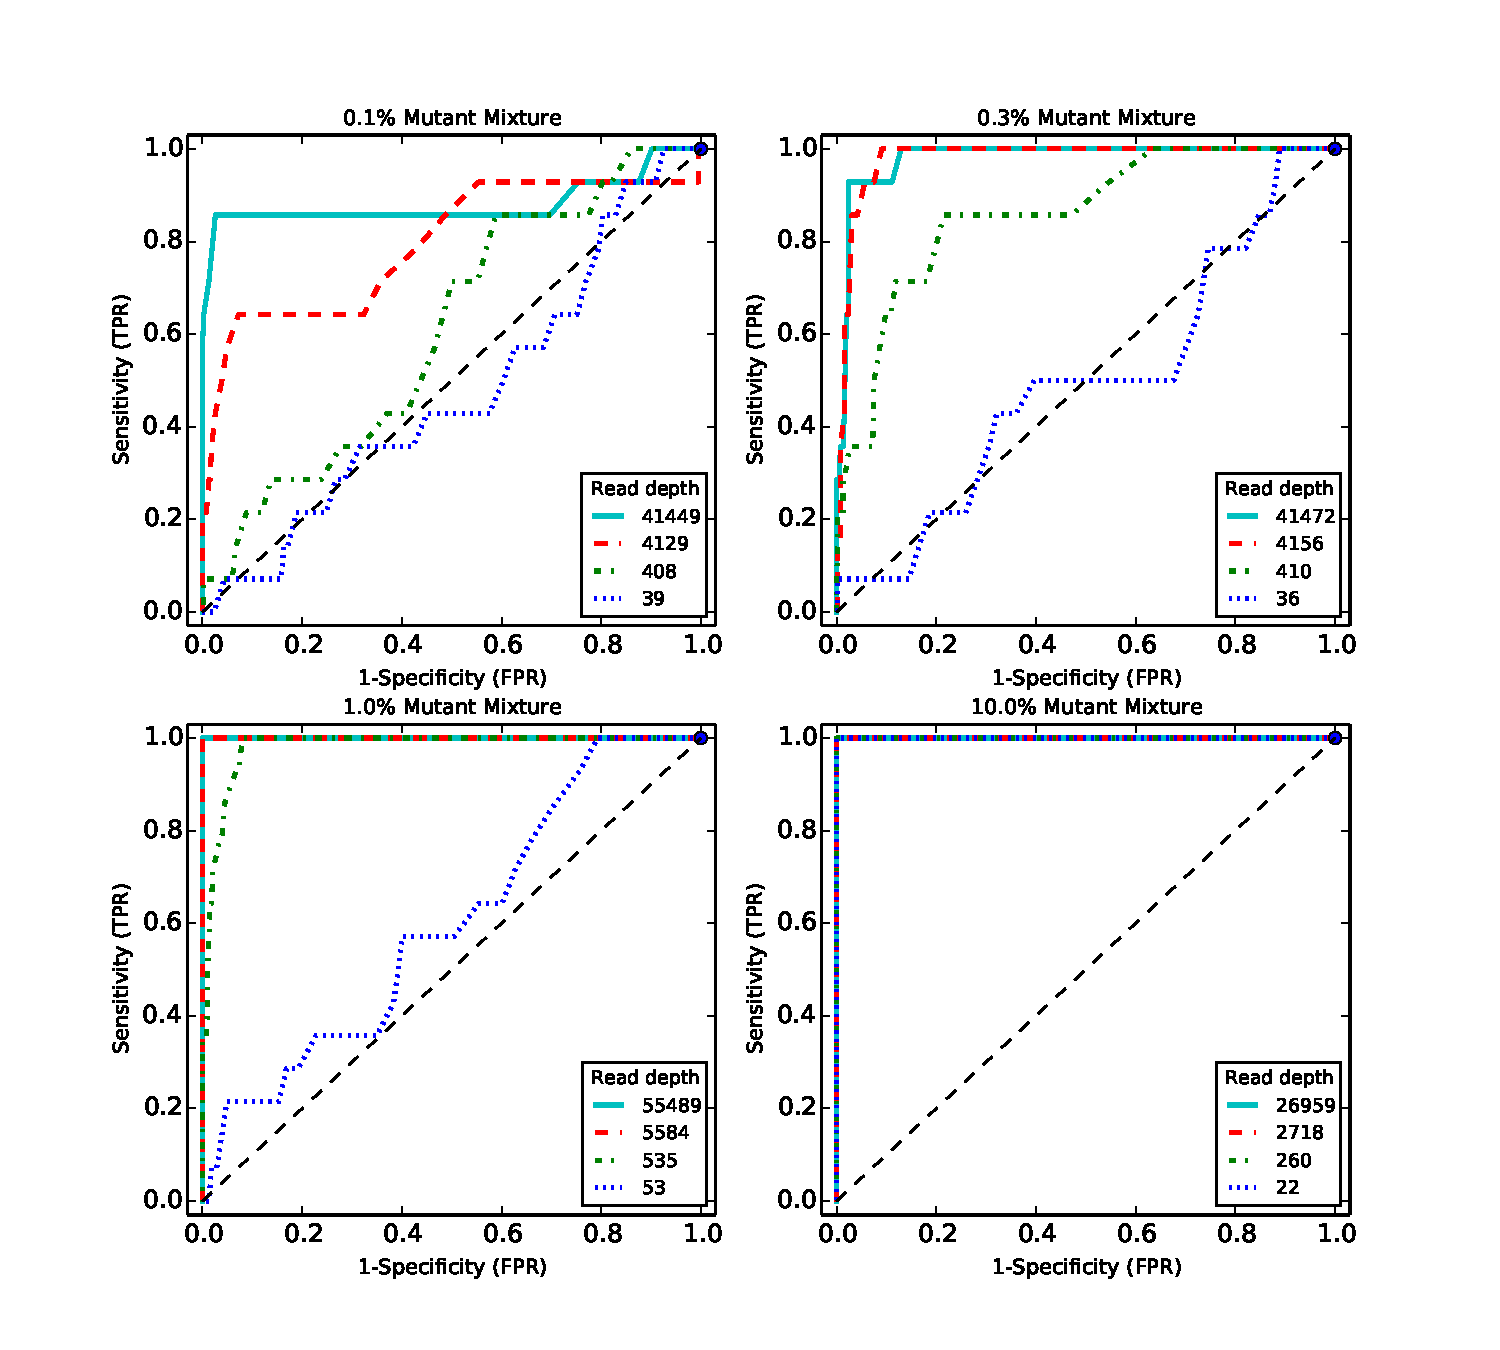
\includegraphics[width=120mm]{figs/ROC_without_chi2_jeffrey.pdf}
\caption{ROC curve varying read depth showing detection performance.}
\label{fig:ROC_jeffrey}
\end{center}
\end{figure}


\begin{figure}[htbp]
\begin{center}
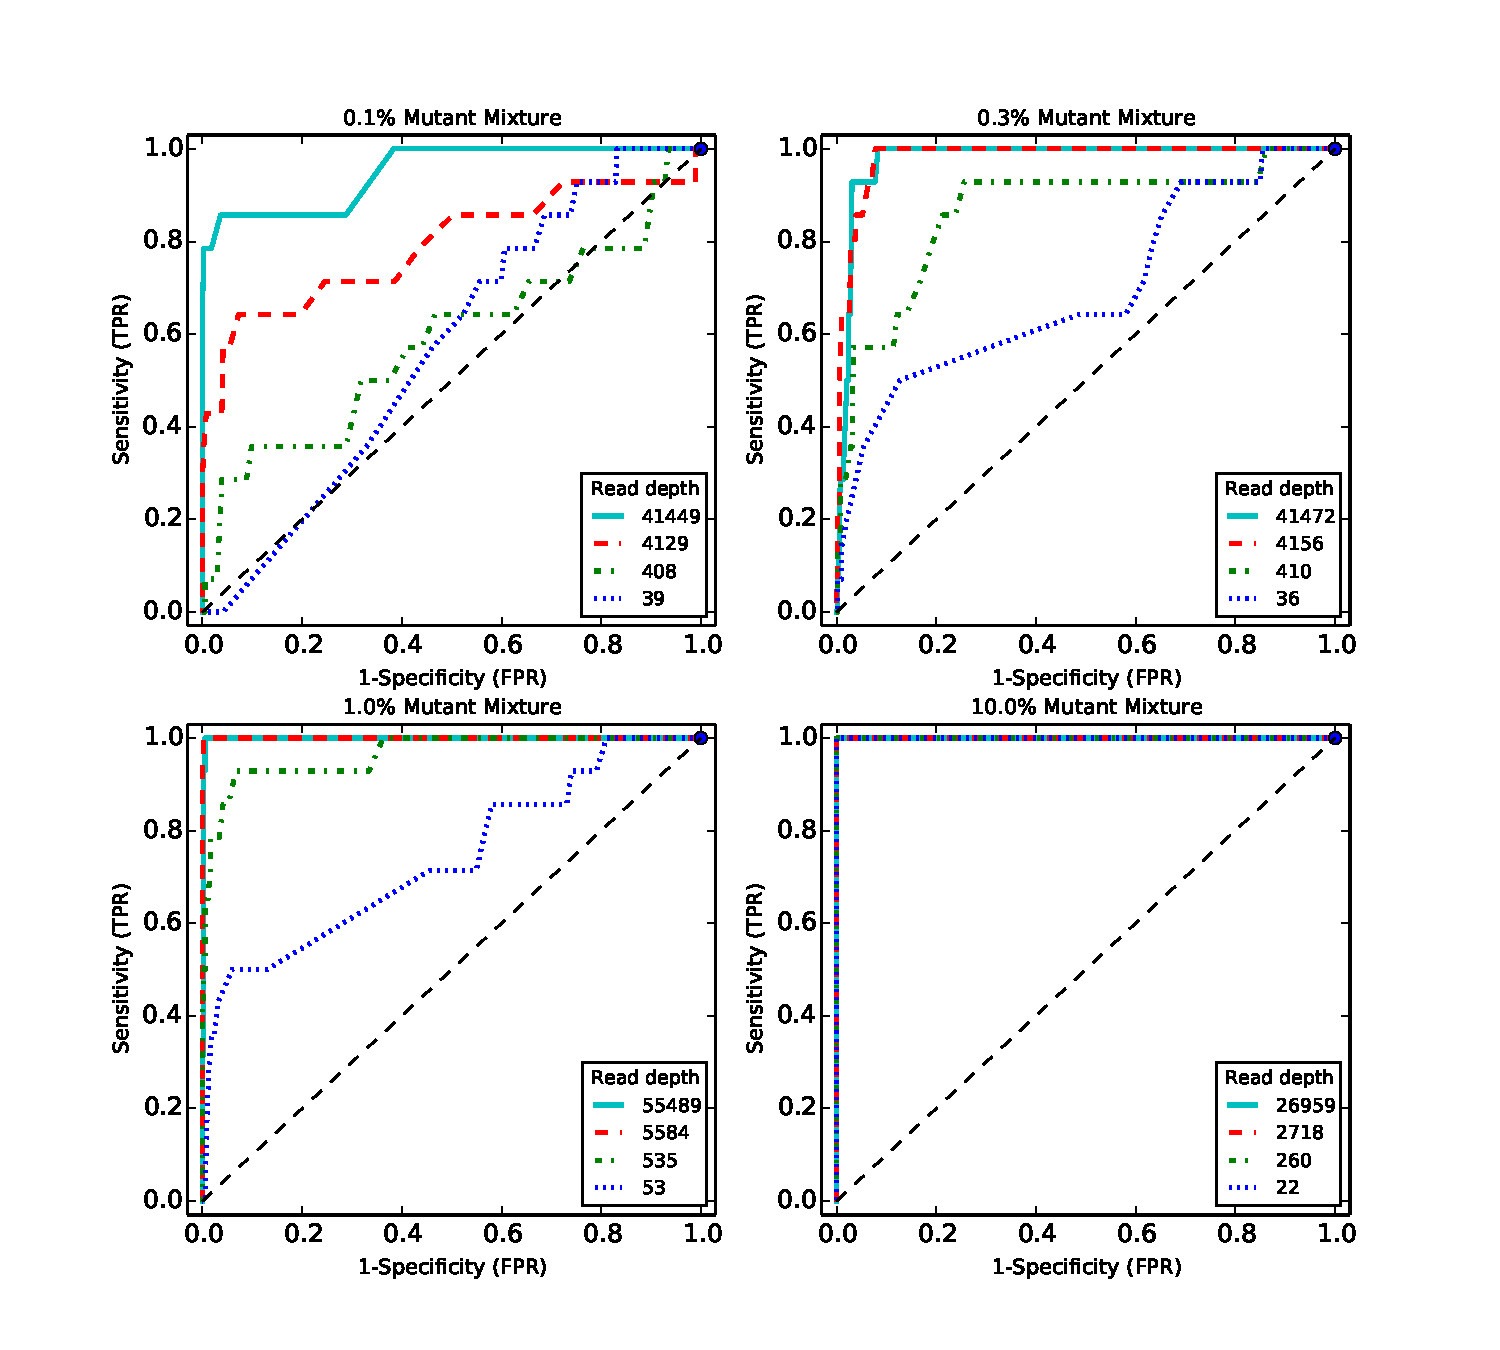
\includegraphics[width=120mm]{figs/ROC_without_chi2_lognormal.pdf}
\caption{ROC curve varying read depth showing detection performance.}
\label{fig:ROC_lognormal}
\end{center}
\end{figure}

\begin{figure}[h]
\begin{center}
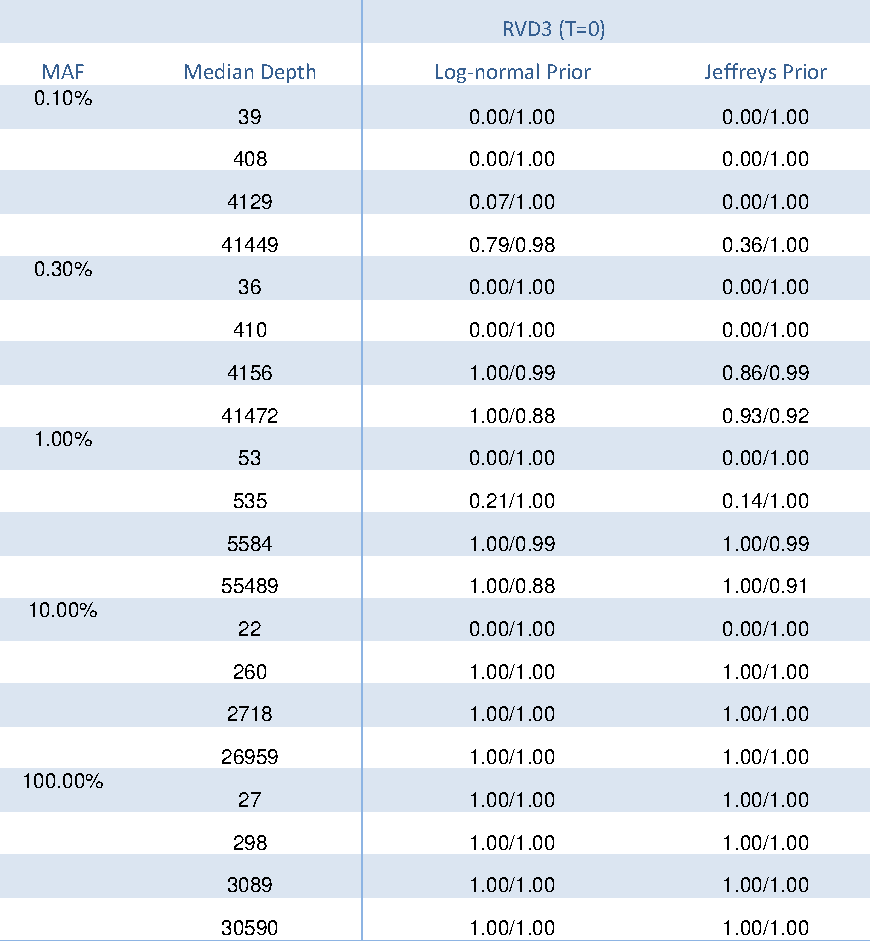
\includegraphics[width=160mm]{tables/Sen_Speci.pdf}
\caption{Sensitivity/Specificity comparison of RVD3 with different priors.}
\label{tbl:SS}
\end{center}
\end{figure}

\begin{figure}[h]
\begin{center}
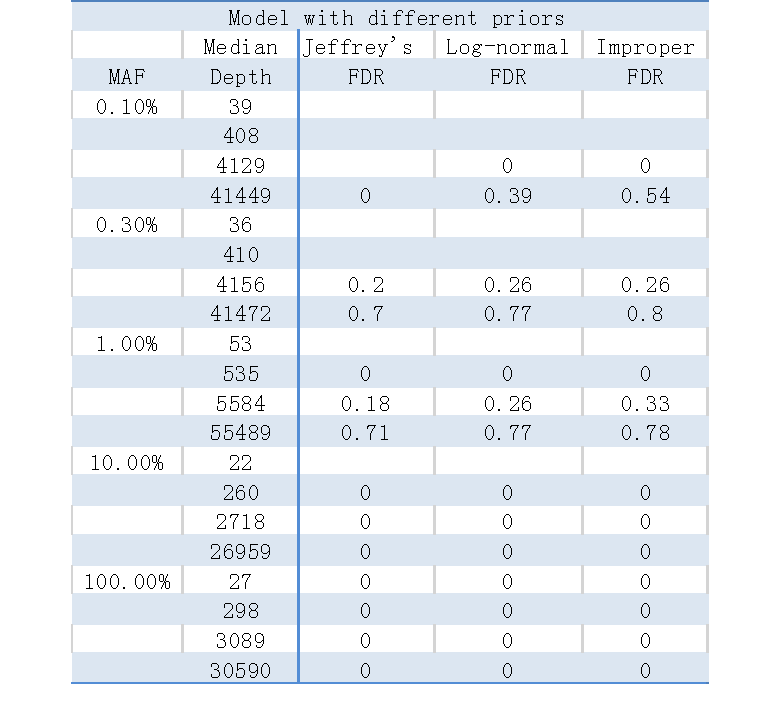
\includegraphics[width=160mm]{tables/FDR.pdf}
\caption{Sensitivity/Specificity comparison of RVD3 with different priors.}
\label{tbl:FDR}
\end{center}
\end{figure}

\subsubsection{Sensitivity/Specificity/FDR}

Figure~\ref{tbl:SS} shows that the sensitivity and specificity of the RVD3 of different priors compared with the model without priors. Log-normal prior shows a higher sensitivity and specificity value than the Jeffreys prior.
Figure~\ref{tbl:FDR} shows the false discovery rate of the RVD3 with different priors. Jeffreys prior shows a smaller false discovery rate and higher accuracy than others. It is obvious no matter which pirors, the variant detection performance acquires lower FDR than the model without priors. Based on the various advantages for Jeffreys and log-normal prior, RVD3 can afford a more appropariate choice for the precision prior. Here we chose Jeffreys prior because it needs more attention to false discovery rate and accuracy for variants calling research, compared with the clinical experiment or diagnosis which cares more on true positive rate and true negative rate.
%%%%%%%%%%%%%%%%%%%%%%%%%%%%%%
% Results of Jeffreys prior on yeast data
%%%%%%%%%%%%%%%%%%%%%%%%%%%%%%
\subsection{Results of Jeffreys prior on yeast data}

We demonstrated our RVD3 model with Jeffreys piror on yeast data to identify the variants.


%%%%%%%%%%%%
% Discussion
%%%%%%%%%%%%
\section{Discussion}


\appendix

%%%%%%%%%%%%%%%%%%%
% Appendix A: Parameter Initialization
%%%%%%%%%%%%%%%%%%%
\section{Parameter Initialization}\label{sec:appendix_mom}
Since $r_{ji} \thicksim \text{Binomial}(n_{ji}, \theta_{ji})$, the first population moment is  $E[r_{ji}] = \theta_{ji} n_{ji}$ and the first sample moment is simply $m_1 = r_{ji}$. Therefore the MoM estimator is
\begin{equation}
	\tilde{\theta}_{ji} = \frac{r_{ji}} {n_{ji}}
\end{equation}

We take the MoM estimate, $\tilde{\theta}_{ji}$, as data for the next conditional distribution in the hierarchical model. The distribution is $\theta_{ji} \thicksim \text{Beta}(\mu_jM_j, (1-\mu_j)M_j)$. The first and second population moments are
\begin{eqnarray}
	E[\theta_{ji}] =& \mu_j,\\
	\text{Var}[\theta_{ji}] =& \frac{\mu_j(1-\mu_j)} { M_j + 1 }.
\end{eqnarray}
The first and second sample moments are $m_1 = \frac{1}{N}\sum_{i=1}^N \theta_{ji}$ and $m_2 = \frac{1}{N}\sum_{i=1}^N \theta_{ji}^2$. Setting the population moments equal to the sample moments and solving for $\mu_j$ and $M_j$ gives
\begin{eqnarray}
	\tilde{\mu}_j =& \frac{1}{N} \sum_{i=1}^N \theta_{ji}, \\
	\tilde{M_j} =& \frac{ \tilde{\mu}_j (1 - \tilde{\mu}_j ) } { \frac{1}{N} \sum_{i=1}^N \theta_{ji}^2 } -1.
\end{eqnarray}

Following the same procedure for the parameters of $\mu_j \thicksim \text{Beta}(\mu_0, M_0)$ gives the following MoM estimates
\begin{eqnarray}
	\tilde{\mu}_0 =& \frac{1}{J} \sum_{j=1}^J \mu_j \\
	\tilde{M}_0 =& \frac{ \tilde{\mu}_0 (1 - \tilde{\mu}_0 ) } {\frac{1}{J} \sum_{j=1}^J \mu_j^2 } -1.
\end{eqnarray}

%%%%%%%%%%%%%%%%%%%
% Appendix B: Comparison Statistics
%%%%%%%%%%%%%%%%%%%


\bibliographystyle{apalike}
\bibliography{bioinfo}
\end{document}
